A Figura \ref{fig:rolamento} representa os esforços no rolamento.

\begin{figure}[H]
  \centering
  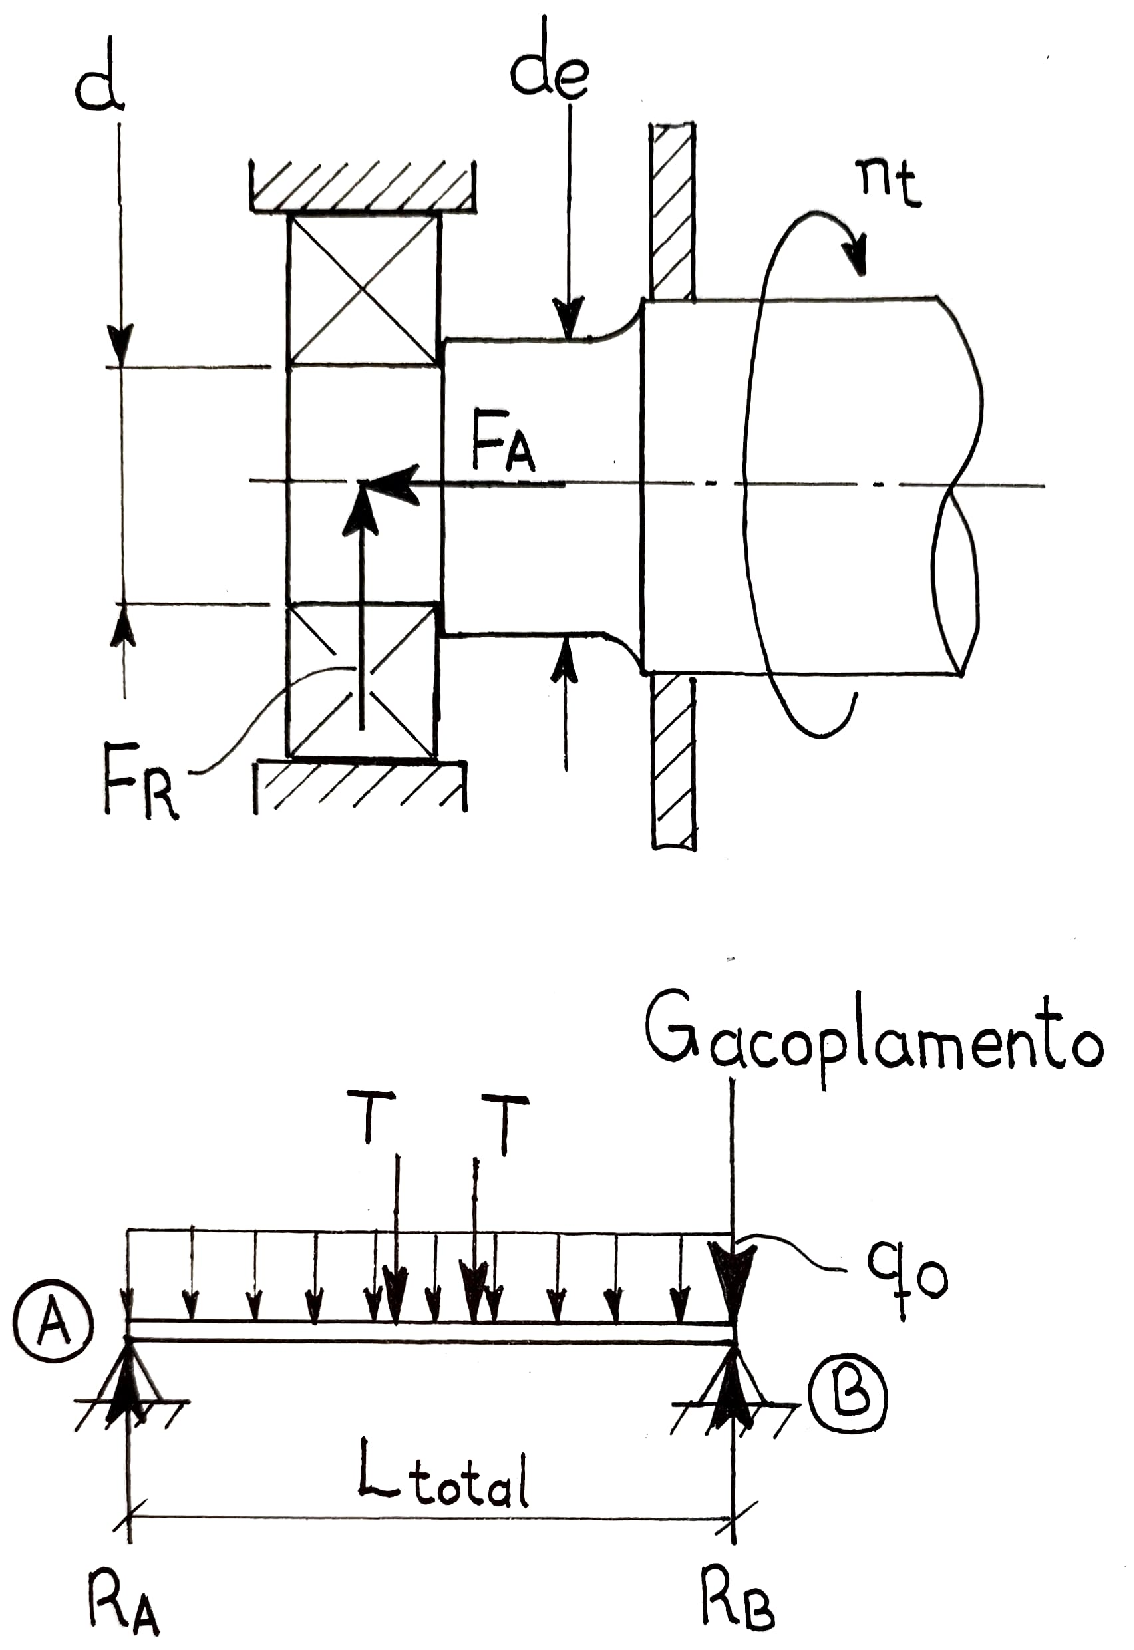
\includegraphics[width=0.5\textwidth]{content/sections/03_sistema_de_elevacao/sections/05_projeto_do_eixo_do_tambor/sections/03_selecao_de_rolamento/figures/rolamento.pdf}
  \caption{Representação dos esforços no rolamento (Autor)}
  \label{fig:rolamento}
\end{figure}


A força radial é dada pela reação de apoio no ponto A, obtida na modelagem estática do tambor (Tabela \ref{tab:dados_esforcos_tambor}), sendo $F_R = R_A = \boxed{\SI{28025.68}{\newton}}$.

A força axial é dada pela equação:

\begin{equation}
  F_A = \num{0.2} \cdot F_R
  \label{eq:forca_axial}
\end{equation}

\begin{align*}
  F_A & = \num{0.2} \cdot \num{28025.68} \\
  F_A & = \boxed{\SI{5605.14}{\newton}}
\end{align*}

A carga estática equivalente é dada pela equação:

\begin{equation}
  P_0 = F_R + Y_0 \cdot F_A
  \label{eq:carga_estatica}
\end{equation}

O rolamento adotado é um \textbf{rolamento autocompensador de rolos}. Os fatores de cálculo foram obtidos no catálogo da SKF \cite{skf_rolamentos}, consultando as tabelas abaixo:

\begin{figure}[H]
  \centering
  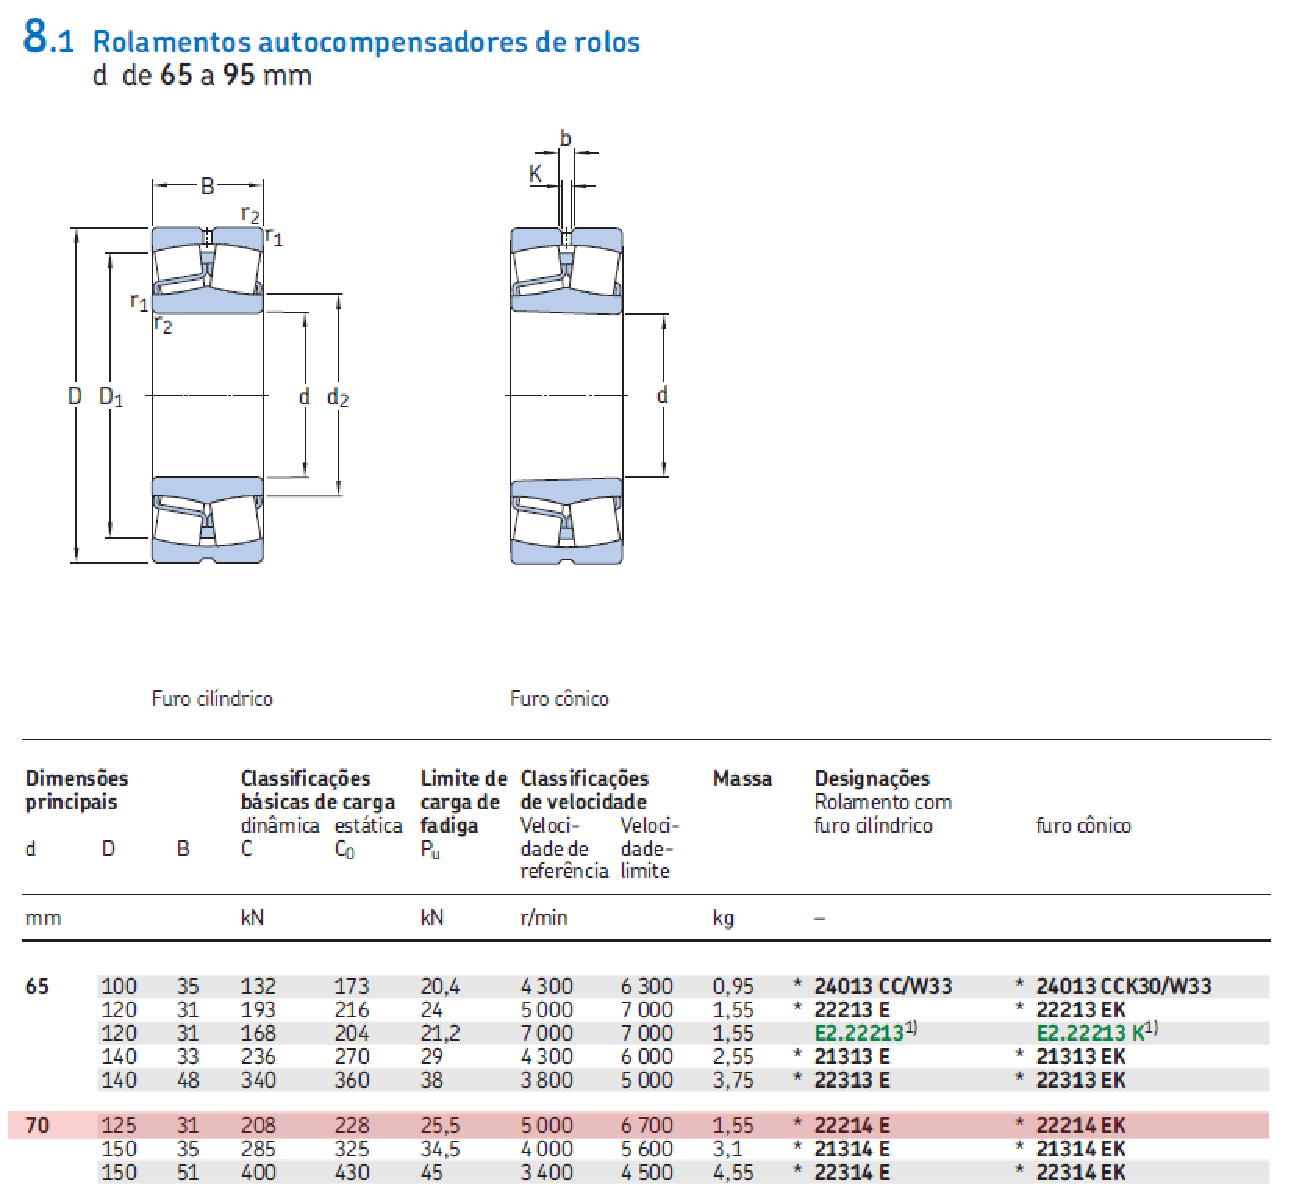
\includegraphics[width=1\textwidth]{content/sections/03_sistema_de_elevacao/sections/05_projeto_do_eixo_do_tambor/sections/03_selecao_de_rolamento/figures/rolamento_catalogo.pdf}
  \caption{Catálogo de rolamentos \cite[p.~906]{skf_rolamentos}}
  \label{fig:rolamento_catalogo}
\end{figure}

\begin{figure}[H]
  \centering
  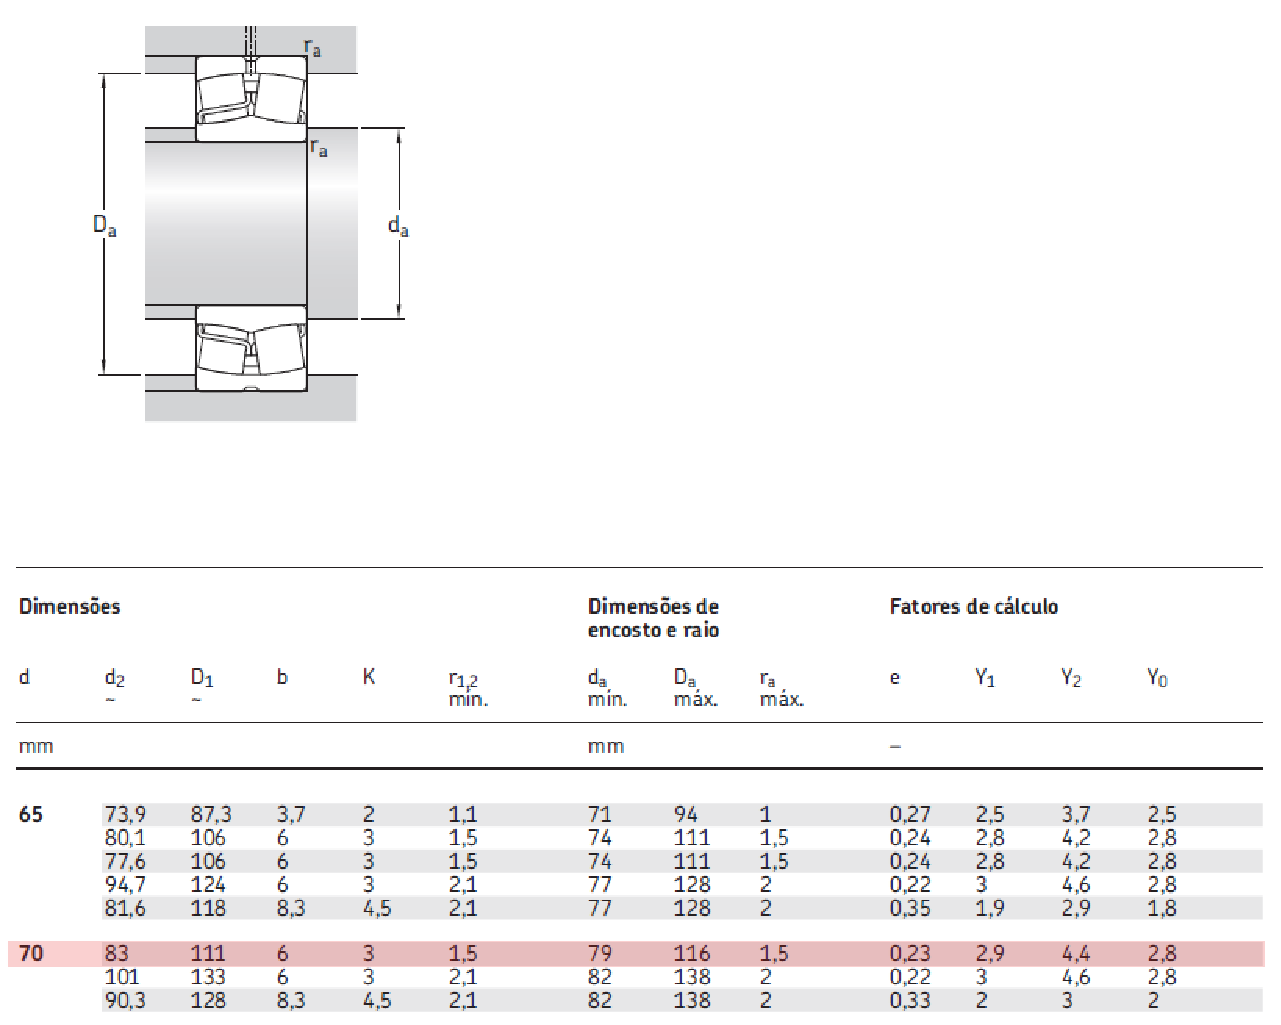
\includegraphics[width=1\textwidth]{content/sections/03_sistema_de_elevacao/sections/05_projeto_do_eixo_do_tambor/sections/03_selecao_de_rolamento/figures/rolamento_fatores.pdf}
  \caption{Catálogo de rolamentos \cite[p.~907]{skf_rolamentos}}
  \label{fig:rolamento_fatores}
\end{figure}

Os dados obtidos foram:

\begin{table}[H]
  \centering
  \caption{Dados do rolamento adotado conforme o catálogo da SKF}
  \label{tab:dados_obtidos_rolamento}
  \begin{tabularx}{\textwidth}{>{\centering\arraybackslash}X>{\centering\arraybackslash}X>{\centering\arraybackslash}X}
    \toprule
    Parâmetro                  & Símbolo              & Valor                  \\
    \midrule
    Modelo do rolamento        & -                    & 22214E                 \\
    Carga dinâmica             & $C$                  & \SI{208}{\kilo\newton} \\
    Carga estática             & $C_0$                & \SI{228}{\kilo\newton} \\
    Rotação máxima             & $n_{\text{max}}$     & \SI{6700}{\rpm}        \\
    Massa                      & $m$                  & \SI{1.55}{\kilo\gram}  \\
    Diâmetro do encosto mínimo & $d_{a_{\text{min}}}$ & \SI{79}{\milli\meter}  \\
    Diâmetro da pista interna  & $d_2$                & \SI{83}{\milli\meter}  \\
    -                          & $e$                  & \num{0.23}             \\
    -                          & $Y_1$                & \num{2.9}              \\
    -                          & $Y_2$                & \num{4.4}              \\
    -                          & $Y_0$                & \num{2.8}              \\
    \bottomrule
  \end{tabularx}
\end{table}

Verificando a condição do diâmetro do eixo:

\begin{align*}
   & d_{a_{\text{min}}} \leq d_e \leq d_2                                                              \\
   & \SI{79}{\milli\meter} \leq \SI{80}{\milli\meter} \leq \SI{83}{\milli\meter} \rightarrow \text{OK}
\end{align*}

Substituindo os valores na equação \ref{eq:carga_estatica}:

\begin{align*}
  P_0 & = \num{28.03} + \num{2.8} \cdot \num{5.61} \\
  P_0 & = \boxed{\SI{43.74}{\kilo\newton}}
\end{align*}

O fator de segurança para carga estática é dado pela equação:

\begin{equation}
  S_0 = \frac{C_0}{P_0} \geq \num{1.5}
  \label{eq:fator_seguranca_estatica}
\end{equation}

\begin{align*}
  S_0 & = \frac{\num{228}}{\num{43.74}}                           \\
  S_0 & = \boxed{\num{5.21}} \geq \num{1.5} \rightarrow \text{OK}
\end{align*}

A carga dinâmica equivalente é dada pela equação:

\[
  P =
  \begin{cases}
    F_R + Y_1 \cdot F_A                  & \frac{F_A}{F_R} \leq e \\
    \num{0.67} \cdot F_R + Y_2 \cdot F_A & \frac{F_A}{F_R} > e    \\
  \end{cases}
\]

\begin{align*}
  \frac{F_A}{F_R} & = \frac{\num{5.61}}{\num{28.03}} \\
  \frac{F_A}{F_R} & = \num{0.20} \leq e
\end{align*}

Portanto, a carga dinâmica equivalente é dada por:

\begin{equation}
  P = F_R + Y_1 \cdot F_A
  \label{eq:carga_dinamica_equivalente}
\end{equation}

\begin{align*}
  P & = \num{28.03} + \num{2.9} \cdot \num{5.61} \\
  P & = \boxed{\SI{44.3}{\kilo\newton}}
\end{align*}

A vida útil do rolamento é dada pela equação:

\begin{equation}
  L_{10_h} = \frac{10^6}{60 \cdot n} \cdot \left( \frac{C}{P} \right)^{10/3}
  \label{eq:vida_util_rolamento}
\end{equation}

Onde:

\begin{itemize}
  \item $L_{10_h}$: vida útil do rolamento em \si{\hour}.
  \item $n$: rotação do tambor em \si{\rpm} \eqref{eq:rotacao_do_tambor}.
  \item $C$: carga dinâmica do rolamento em \si{\kilo\newton}.
  \item $P$: carga dinâmica equivalente do rolamento em \si{\kilo\newton}.
\end{itemize}

Substituindo os valores na equação \ref{eq:vida_util_rolamento}:

\begin{align*}
  L_{10_h} & = \frac{10^6}{60 \cdot \num{10.79}} \cdot \left( \frac{\num{208}}{\num{44.3}} \right)^{\frac{10}{3}} \\
  L_{10_h} & = \boxed{\SI{267727}{\hour}}
\end{align*}

Verificando a condição de vida útil com base no requisito de 3200 horas (Tabela \ref{tab:dados_do_projeto}):

\begin{align*}
  L_{10_h}           & \geq 3200 \text{ h}                       \\
  \SI{267727}{\hour} & \geq 3200 \text{ h} \rightarrow \text{OK}
\end{align*}
